\documentclass[12pt]{article}

% Packages for nicer formatting
\usepackage{array}      % for better tables
\usepackage{graphicx}   % for including graphics
\usepackage{booktabs}   % professional looking tables
\usepackage{geometry}   % page margins
\geometry{margin=1in}

% Command to define a "fact" entry
\newcommand{\datafact}[2]{%
  \noindent\textbf{#1:} #2 \par
}

\begin{document}


\section*{Data Facts Report - Tate Mason}

\subsection*{Summary}
\datafact{Dataset}{PSID - Labor Outcomes}
\datafact{Time Period}{1999--2017}
\datafact{Unit of Analysis}{Individual-year}

\subsection*{Graphics}
\begin{figure}[h!]
    \centering
    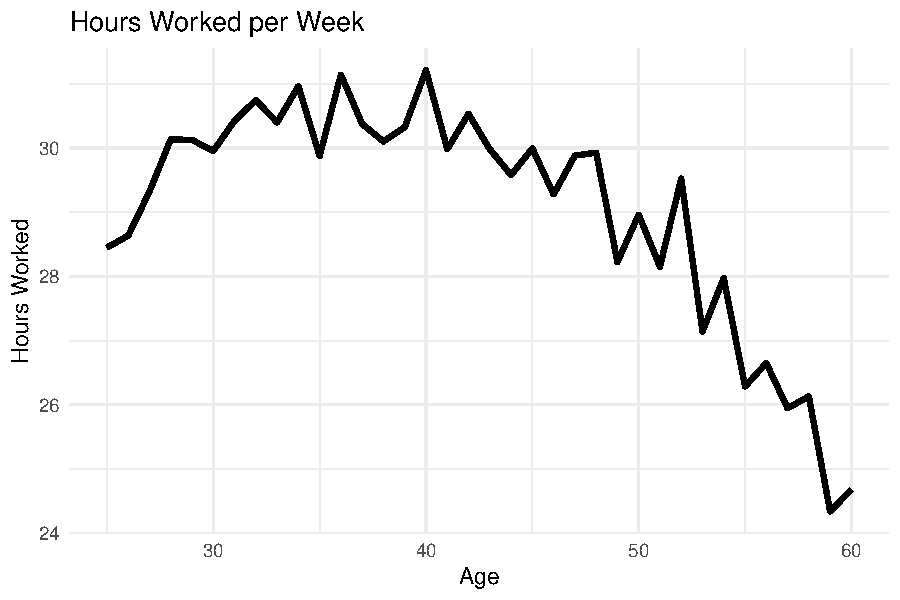
\includegraphics[width=0.8\textwidth]{~/SchoolWork/Y2S1/Macro/PSets/ps1/output/hr_age_fe.pdf}
    \caption{Labor Force Participation Rate by Age (with Age Fixed Effects)}
\end{figure}

As can be seen, in the whole sample, labor force participation peaks around age 50 and begins to decline thereafter, though at a slower rate
than one may expect.

\begin{figure}[h!]
    \centering
    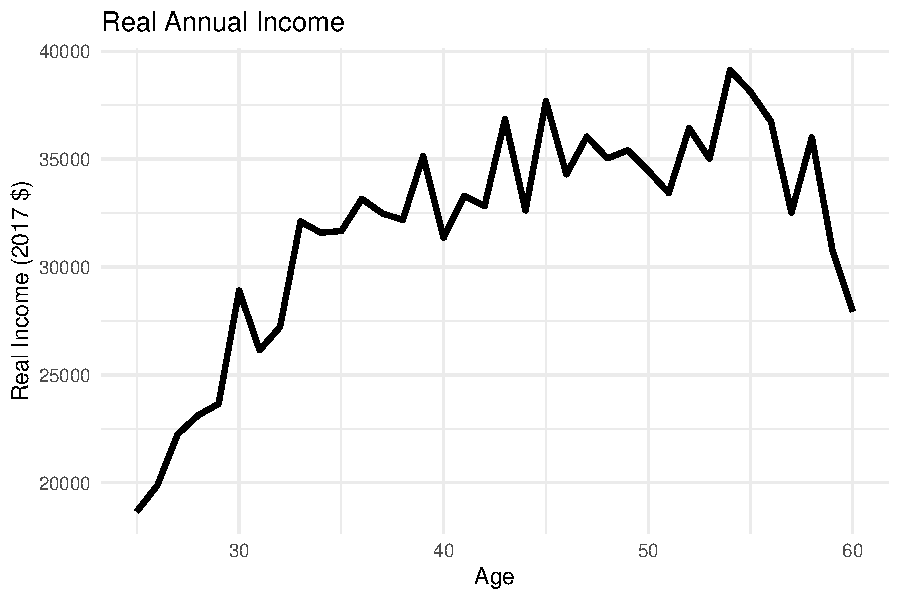
\includegraphics[width=0.8\textwidth]{~/SchoolWork/Y2S1/Macro/PSets/ps1/output/inc_age_fe.pdf}
    \caption{Average Income by Age (with Age Fixed Effects)}
\end{figure}

Average income peaks around age 45-50, which is consistent with the life-cycle hypothesis of income.

\begin{figure}[h!]
    \centering
    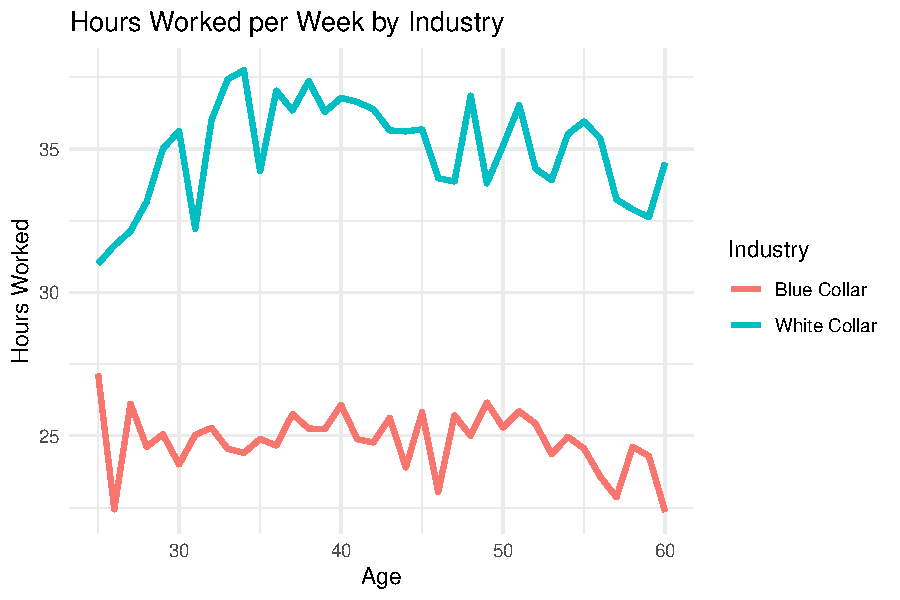
\includegraphics[width=0.8\textwidth]{~/SchoolWork/Y2S1/Macro/PSets/ps1/output/hr_age_fe_ind.pdf}
    \caption{Average Hours Worked by Age (with Age Fixed Effects and Stratified by Industry)}
\end{figure}

Average hours worked follows the hump shape we would expect.

\begin{figure}[h!]
    \centering
    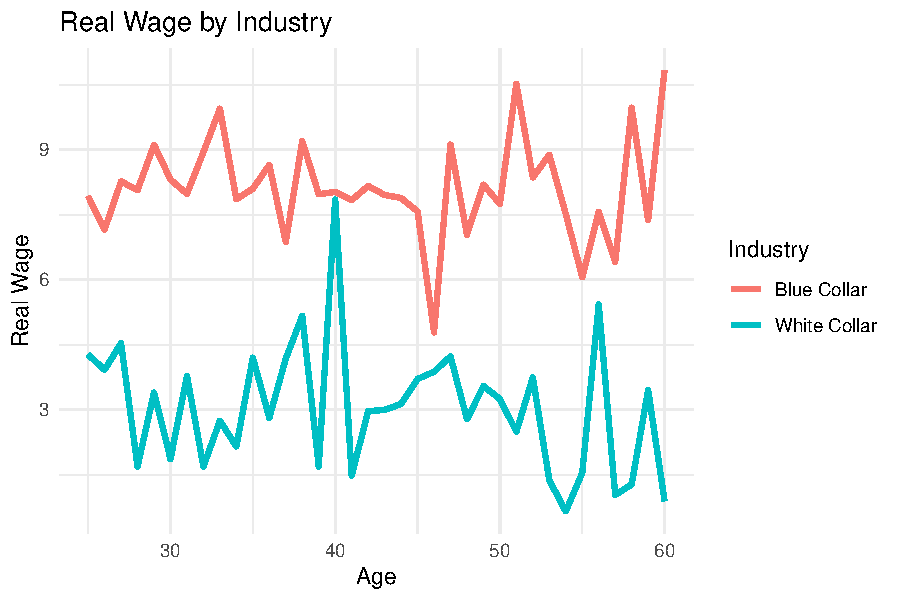
\includegraphics[width=0.8\textwidth]{~/SchoolWork/Y2S1/Macro/PSets/ps1/output/wage_age_fe_ind.pdf}
    \caption{Average Wage by Age (with Age Fixed Effects and Stratified by Industry)}
\end{figure}

Wages are all over the place, but seem to peak between 40-45 before declining.

\begin{figure}[h!]
    \centering
    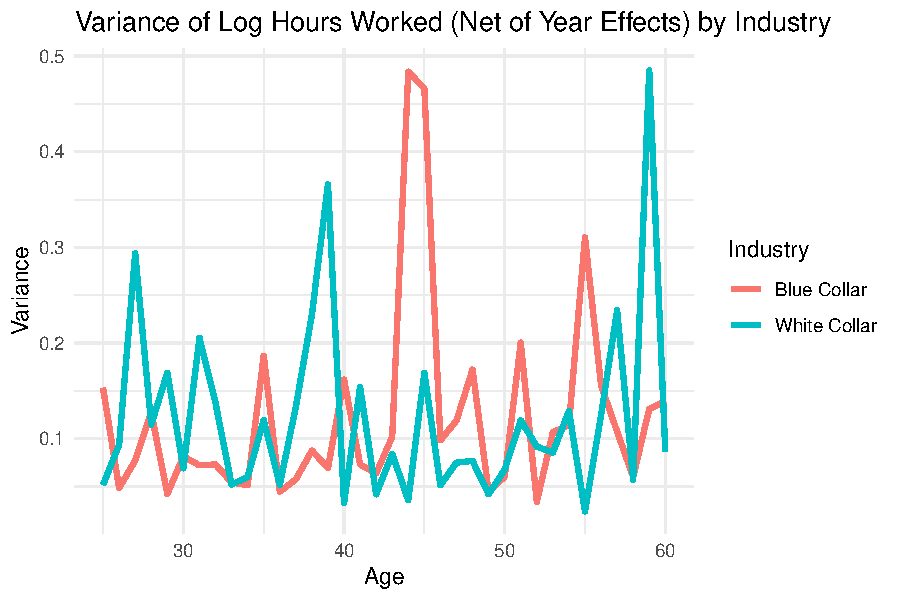
\includegraphics[width=0.8\textwidth]{~/SchoolWork/Y2S1/Macro/PSets/ps1/output/var_hr_age_ind.pdf}
    \caption{Variance of Hours Worked by Age (Stratified by Industry)}
\end{figure}

Variance of hours worked is highest amongst the older members of the sample, showing that there is likely wealth effects at play.

\begin{figure}[h!]
    \centering
    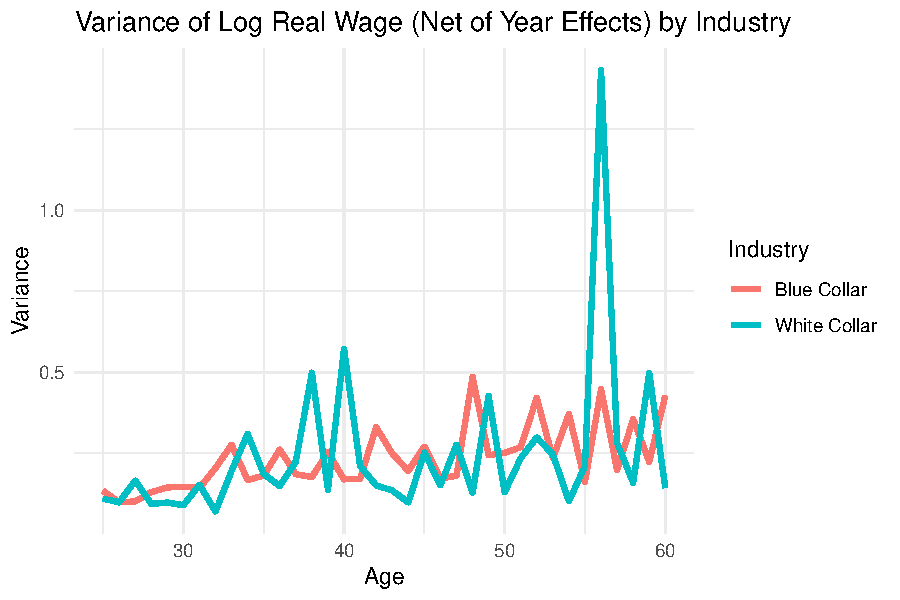
\includegraphics[width=0.8\textwidth]{~/SchoolWork/Y2S1/Macro/PSets/ps1/output/var_wage_age_ind.pdf}
    \caption{Variance of Wages by Age (Stratified by Industry)}
\end{figure}

Variance of wages is mostly stagnant, but is raising slightly with age, spliking at age 40.

\begin{figure}[h!]
    \centering
    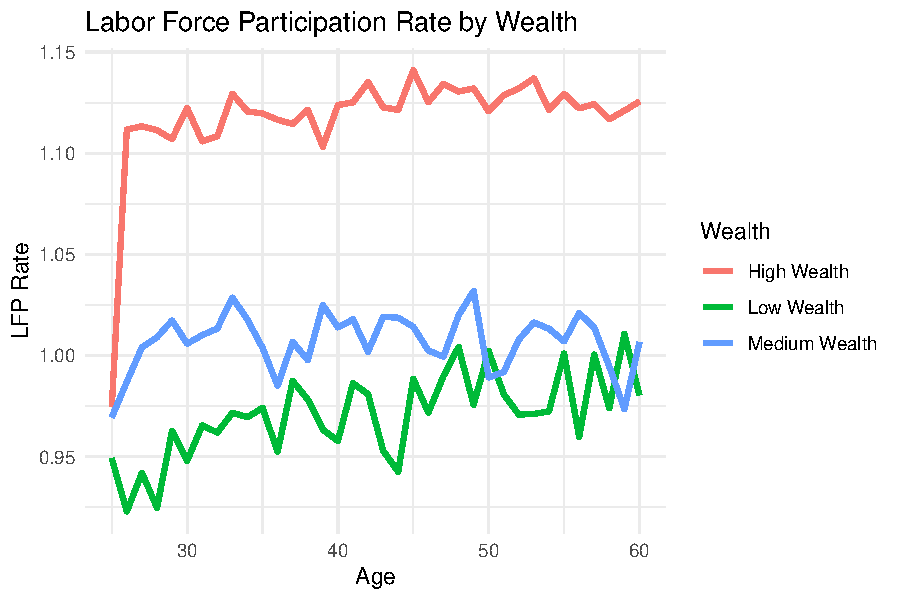
\includegraphics[width=0.8\textwidth]{~/SchoolWork/Y2S1/Macro/PSets/ps1/output/lfp_age_fe_wealth.pdf}
    \caption{Labor Force Participation Rate by Age (with Age Fixed Effects and Stratified by Wealth)}
\end{figure}  

Labor force participation is highest amongst the wealthiest members of the sample, and lowest amongst the poorest.

\begin{figure}[h!]
    \centering
    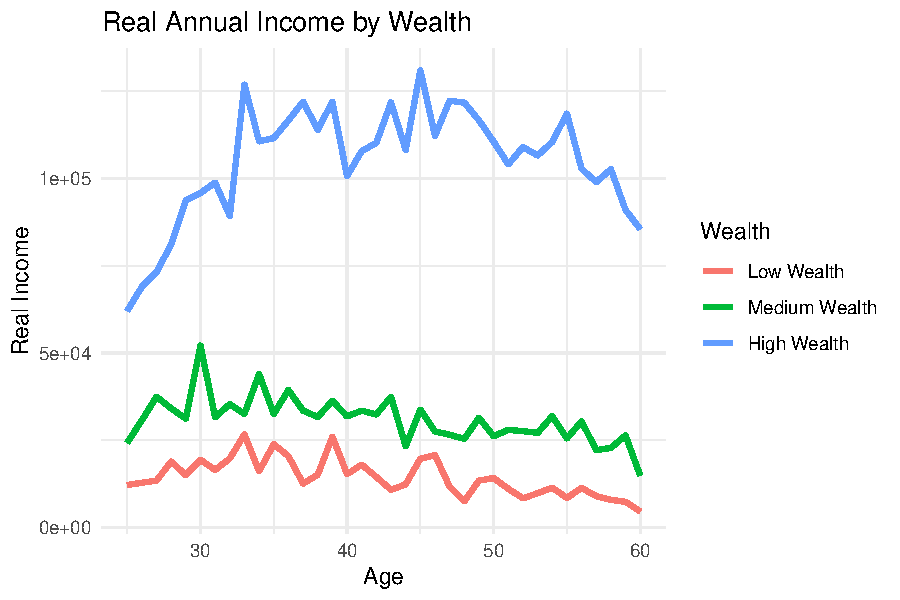
\includegraphics[width=0.8\textwidth]{~/SchoolWork/Y2S1/Macro/PSets/ps1/output/inc_age_fe_wealth.pdf}
    \caption{Average Income by Age (with Age Fixed Effects and Stratified by Wealth)}
\end{figure}
Average income, understandably, is highest amongst the wealthiest members of the sample, and lowest amongst the poorest.

\begin{figure}[h!]
    \centering
    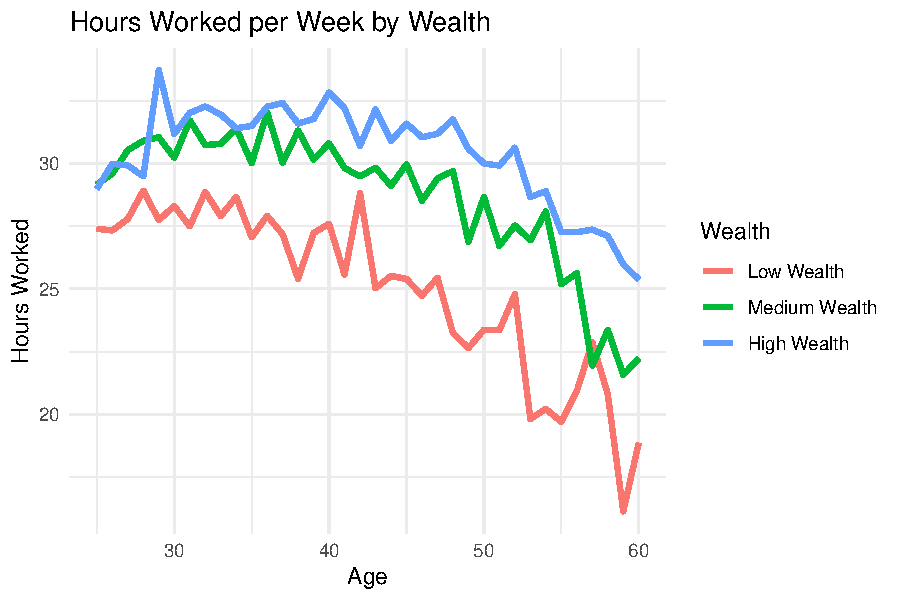
\includegraphics[width=0.8\textwidth]{~/SchoolWork/Y2S1/Macro/PSets/ps1/output/hr_age_fe_wealth.pdf}
    \caption{Average Hours Worked by Age (with Age Fixed Effects and Stratified by Wealth)}
\end{figure}

Average hours worked is highest among wealthiest members of the sample, and lowest amongst the poorest, which perhaps contradicts
the idea that poorer individuals need to work more.

\begin{figure}[h!]
    \centering
    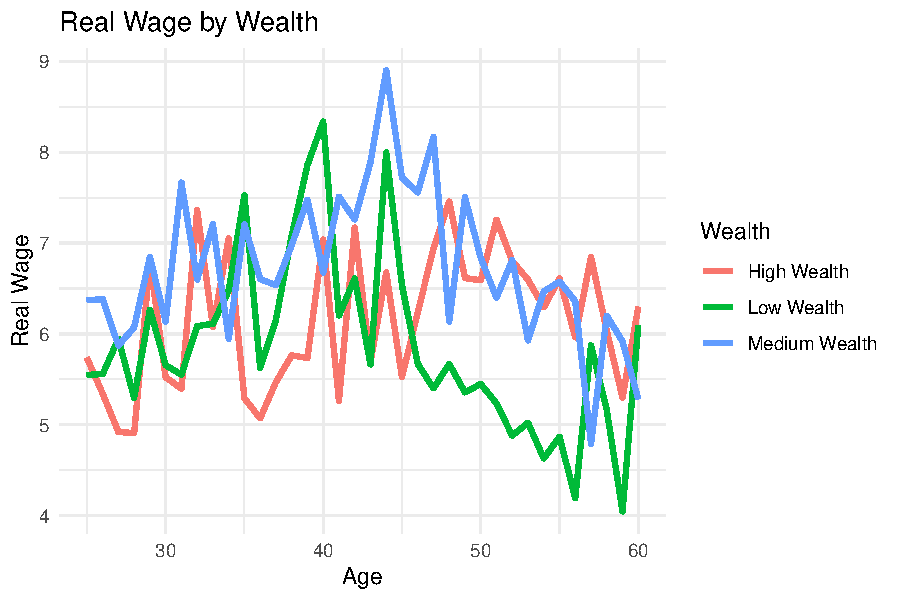
\includegraphics[width=0.8\textwidth]{~/SchoolWork/Y2S1/Macro/PSets/ps1/output/wage_age_fe_wealth.pdf}
    \caption{Average Wage by Age (with Age Fixed Effects and Stratified by Wealth)}
\end{figure}

Again, wages are erratic, but the wealthiest members of the sample seem to have mostly higher wages.

\begin{figure}[h!]
    \centering
    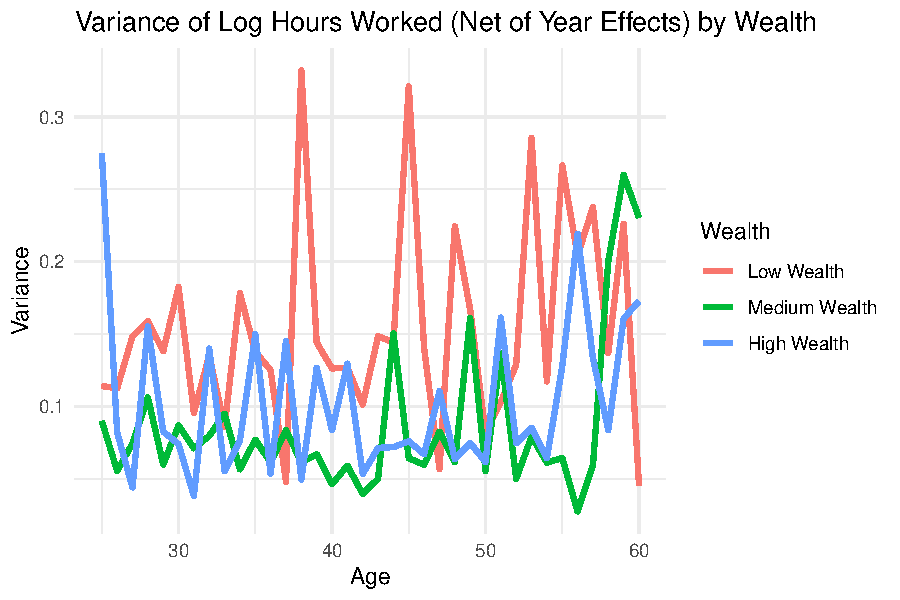
\includegraphics[width=0.8\textwidth]{~/SchoolWork/Y2S1/Macro/PSets/ps1/output/var_hr_age_wealth.pdf}
    \caption{Variance of Hours Worked by Age (Stratified by Wealth)}
\end{figure} 

We see that the poorest members of the sample have the highest variance in hours worked, which may be due
to the need to work more in some years than others or job instability.

\begin{figure}[h!]
    \centering
    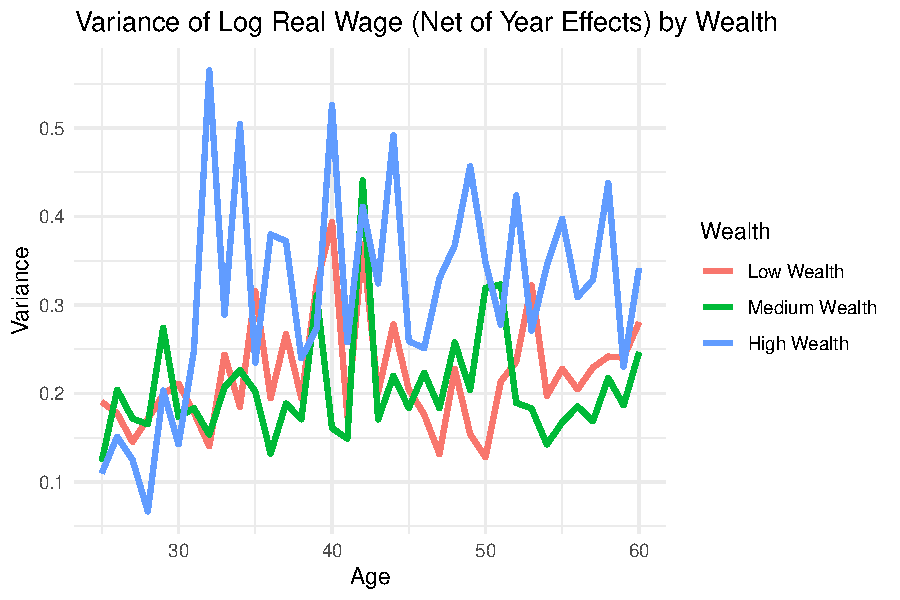
\includegraphics[width=0.8\textwidth]{~/SchoolWork/Y2S1/Macro/PSets/ps1/output/var_wage_age_wealth.pdf}
    \caption{Variance of Wages by Age (Stratified by Wealth)}
\end{figure} 

Variance of wages is highest for the wealthiest members of the sample, which may be due to non-wage income comprising much of their wealth.

\begin{figure}[h!]
    \centering
    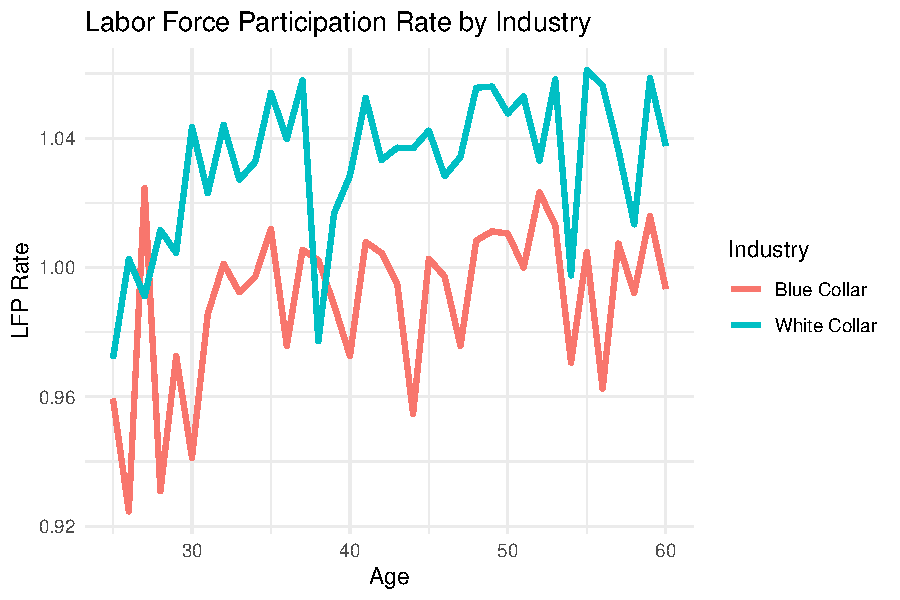
\includegraphics[width=0.8\textwidth]{~/SchoolWork/Y2S1/Macro/PSets/ps1/output/lfp_age_fe_ind.pdf}
    \caption{Labor Force Participation Rate by Age (with Age Fixed Effects and Stratified by Industry)}
\end{figure}

White collar workers have a higher labor force participation rate at nearly all ages, though both groups
follow a similar pattern at different magnitudes.

\begin{figure}[h!]
    \centering
    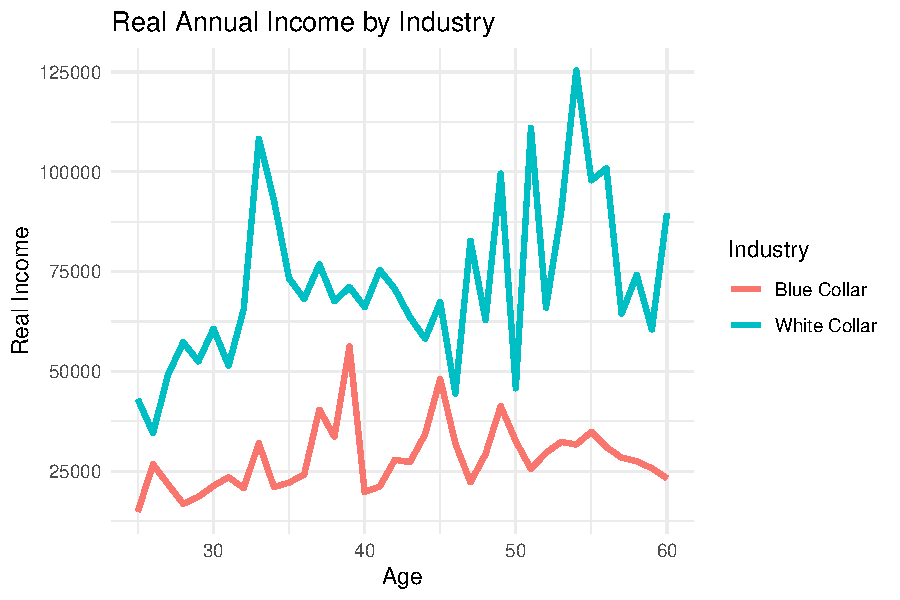
\includegraphics[width=0.8\textwidth]{~/SchoolWork/Y2S1/Macro/PSets/ps1/output/inc_age_fe_ind.pdf}
    \caption{Average Income by Age (with Age Fixed Effects and Stratified by Industry)}
\end{figure}

Average income is higher for white collar workers at all ages, and peaks later for white collar workers.
This may be due to the fact that white collar workers tend to have more opportunities for advancement.

\begin{figure}[h!]
    \centering
    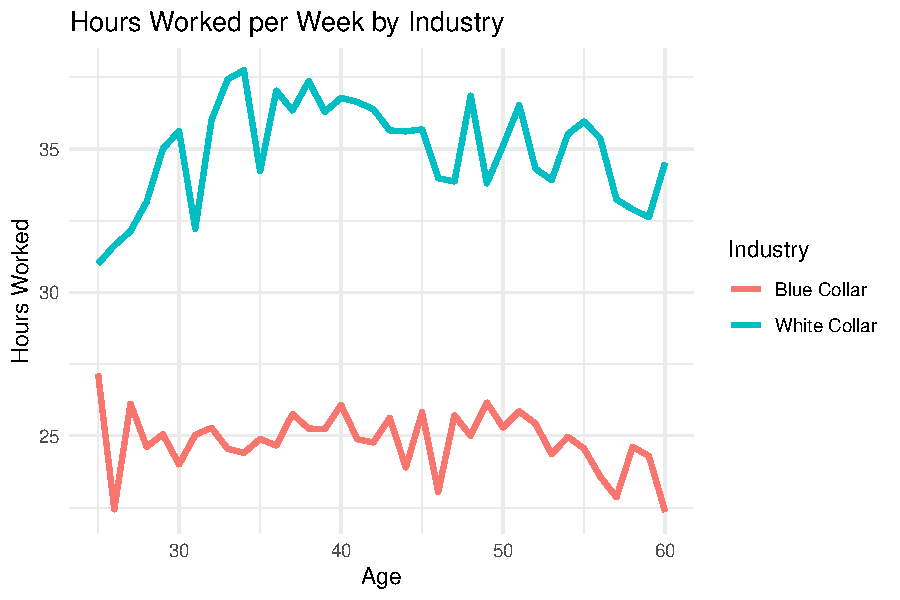
\includegraphics[width=0.8\textwidth]{~/SchoolWork/Y2S1/Macro/PSets/ps1/output/hr_age_fe_ind.pdf}
    \caption{Average Hours Worked by Age (with Age Fixed Effects and Stratified by Industry)}
\end{figure}

White collar workers work more hours at all ages by nearly 20 hours per week, which is a significant difference.
This may be due to blue collar hours being more erratic or blue collar workers having more part-time jobs.

\begin{figure}[h!]
    \centering
    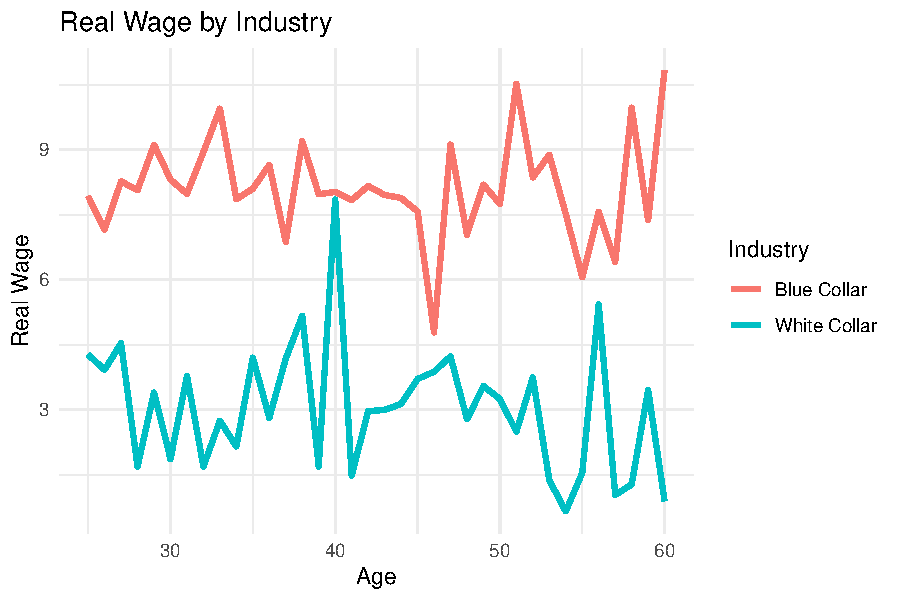
\includegraphics[width=0.8\textwidth]{~/SchoolWork/Y2S1/Macro/PSets/ps1/output/wage_age_fe_ind.pdf}
    \caption{Average Wage by Age (with Age Fixed Effects and Stratified by Wealth)}
\end{figure}

Blue collar workers have a higher average wage at nearly all ages, which is somewhat surprising. This may be due
to the fact that blue collar workers tend to have more unionized jobs, which tend to pay higher wages, or a strange
data quirk.

\begin{figure}[h!]
    \centering
    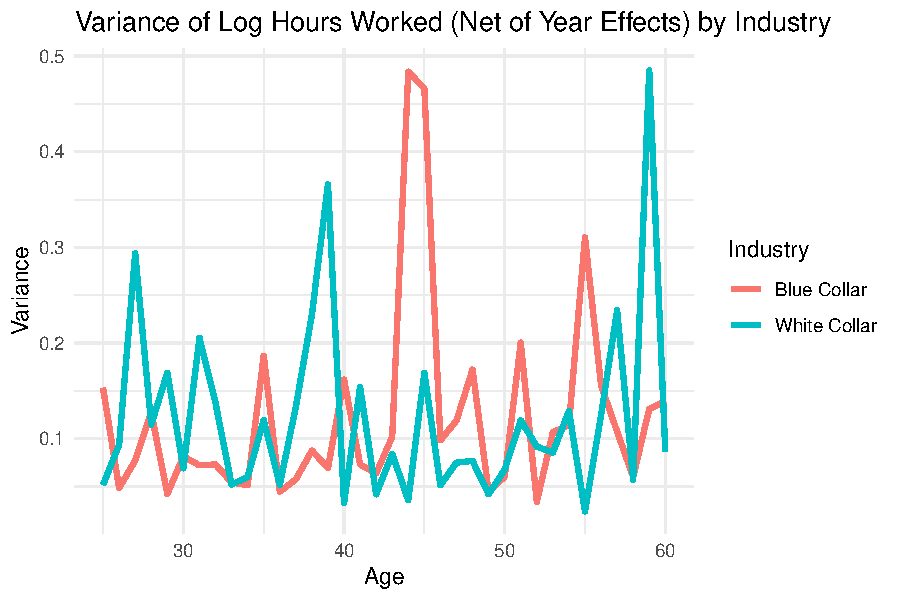
\includegraphics[width=0.8\textwidth]{~/SchoolWork/Y2S1/Macro/PSets/ps1/output/var_hr_age_ind.pdf}
    \caption{Variance of Hours Worked by Age (Stratified by Industry)}
\end{figure}

Variance of hours worked is higher for white collar workers at nearly all ages, which could be attributed to the fact
that white collar workers could have very different hours depending on their job, while blue collar workers tend to have more
consistent hours due to things like union contracts.

\begin{figure}[h!]
    \centering
    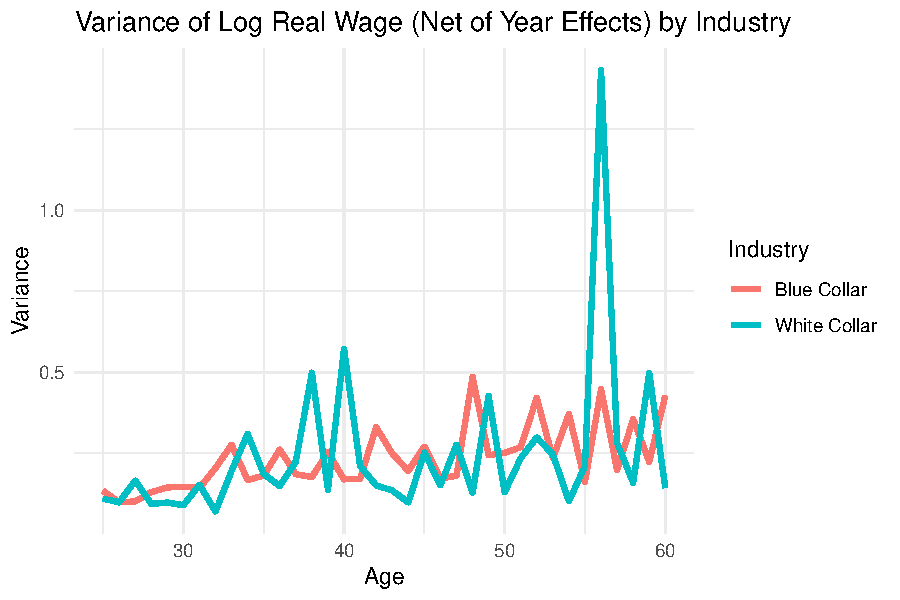
\includegraphics[width=0.8\textwidth]{~/SchoolWork/Y2S1/Macro/PSets/ps1/output/var_wage_age_ind.pdf}
    \caption{Variance of Wages by Age (Stratified by Industry)}
\end{figure}

Variance of wages is mostly in lockstep until age 56 when white collar workers see a one time spike. I cannot hypothesize a
reason for this spike.

\begin{figure}[h!]
    \centering
    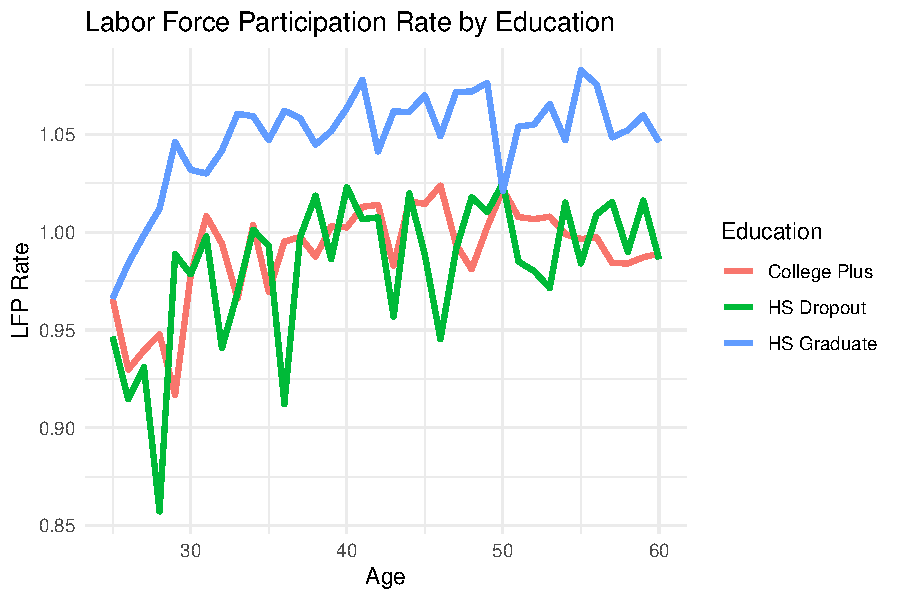
\includegraphics[width=0.8\textwidth]{~/SchoolWork/Y2S1/Macro/PSets/ps1/output/lfp_age_fe_educ.pdf}
    \caption{Labor Force Participation Rate by Age (with Age Fixed Effects and Stratified by Education)}
\end{figure}

Labor force participation is highest for high school graduates who did not attend college, followed by college graduates, and lowest for high school dropouts.
This is somewhat surprising, as one would expect college graduates to have the highest labor force participation rate.

\begin{figure}[h!]
    \centering
    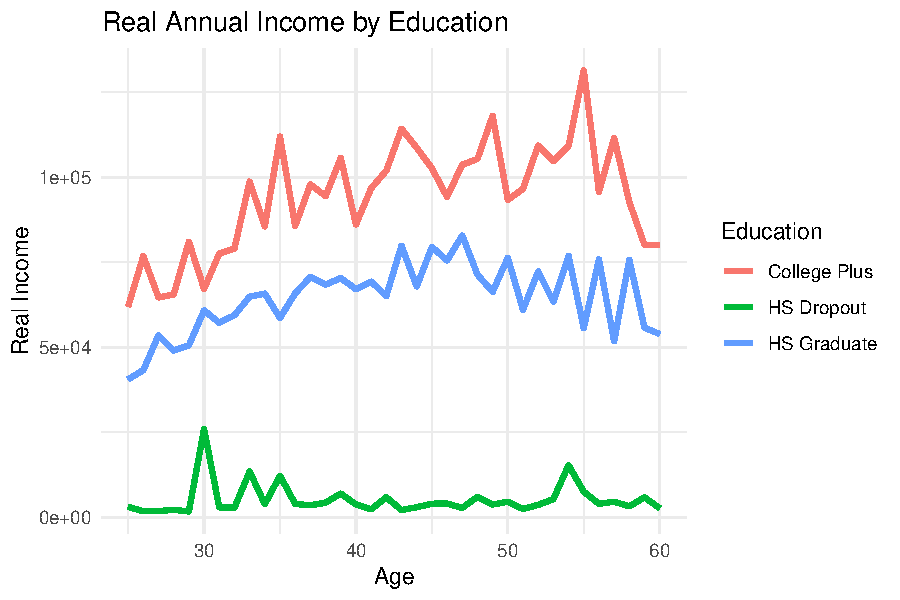
\includegraphics[width=0.8\textwidth]{~/SchoolWork/Y2S1/Macro/PSets/ps1/output/inc_age_fe_educ.pdf}
    \caption{Average Income by Age (with Age Fixed Effects and Stratified by Education)}
\end{figure}

We see that there is a rank order of income by education level, with college graduates earning the most, followed by high school graduates, and then high school dropouts.

\begin{figure}[h!]
    \centering
    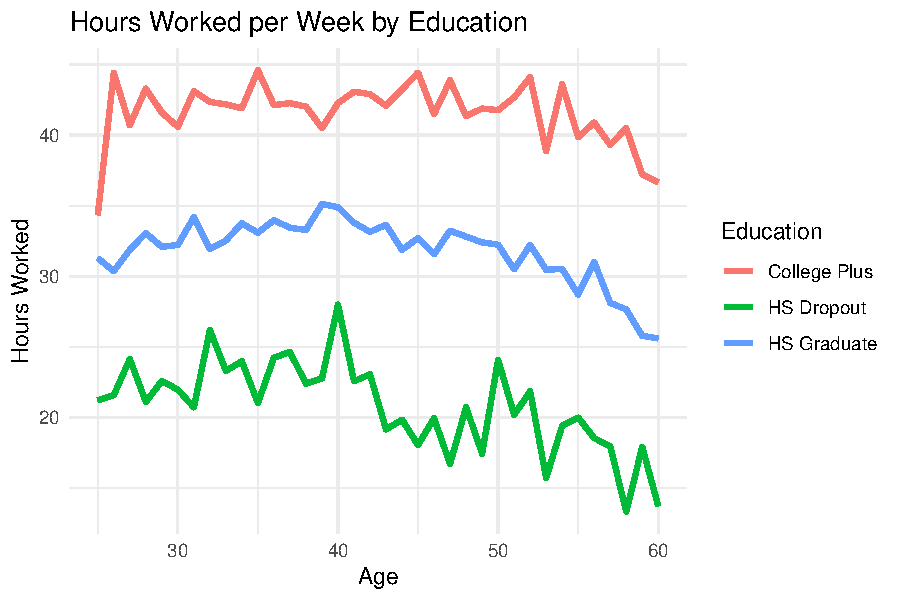
\includegraphics[width=0.8\textwidth]{~/SchoolWork/Y2S1/Macro/PSets/ps1/output/hr_age_fe_educ.pdf}
    \caption{Average Hours Worked by Age (with Age Fixed Effects and Stratified by Education)}
\end{figure}

Hours worked is similarly ranked, with college graduates working the most, followed by high school graduates, and then high school dropouts.

\begin{figure}[h!]
    \centering
    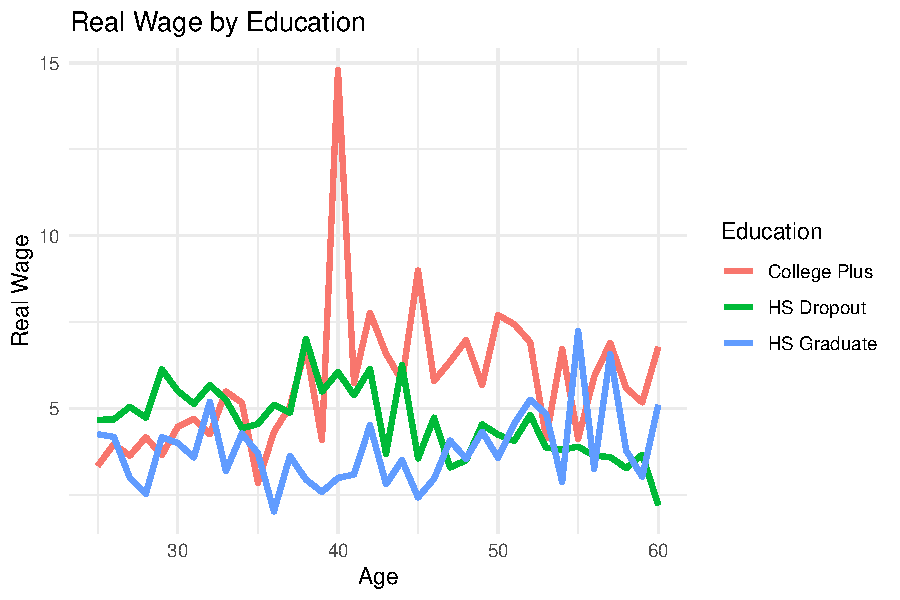
\includegraphics[width=0.8\textwidth]{~/SchoolWork/Y2S1/Macro/PSets/ps1/output/wage_age_fe_educ.pdf}
    \caption{Average Wage by Age (with Age Fixed Effects and Stratified by Education)}
\end{figure} 

Wages are much tighter, with college graduates being in the middle or bottom of the pack until age 40, when they shoot up until joinging the pack again around 55.
  This may be due to college (+) jobs being more erratic in pay early on, but then stabilizing later in life.

\begin{figure}[h!]
    \centering
    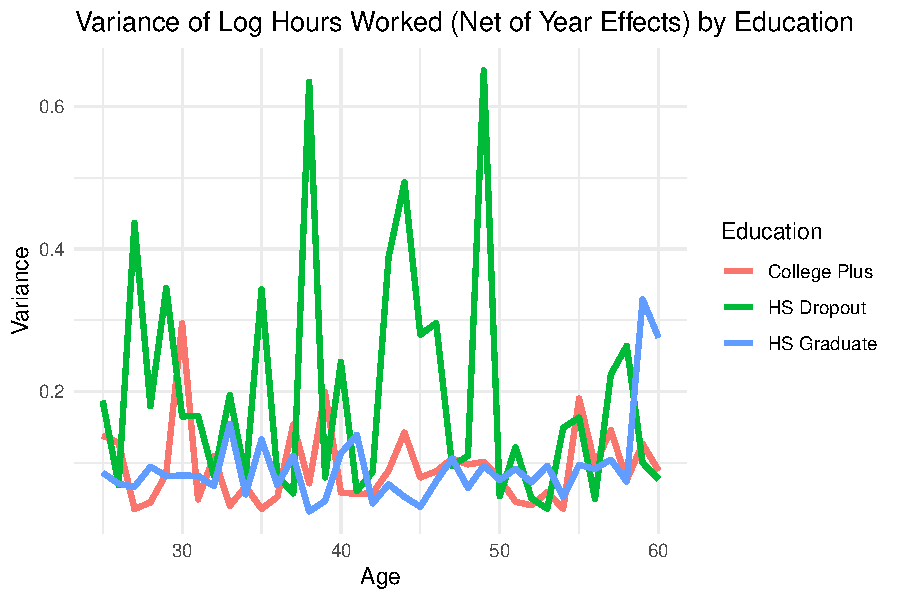
\includegraphics[width=0.8\textwidth]{~/SchoolWork/Y2S1/Macro/PSets/ps1/output/var_hr_age_educ.pdf}
    \caption{Variance of Hours Worked by Age (Stratified by Education)}
\end{figure}

Variance of hours worked is significantly higher for high school dropouts, which is likely due to the fact that they are more likely to have part-time or erratic jobs.

\begin{figure}[h!]
    \centering
    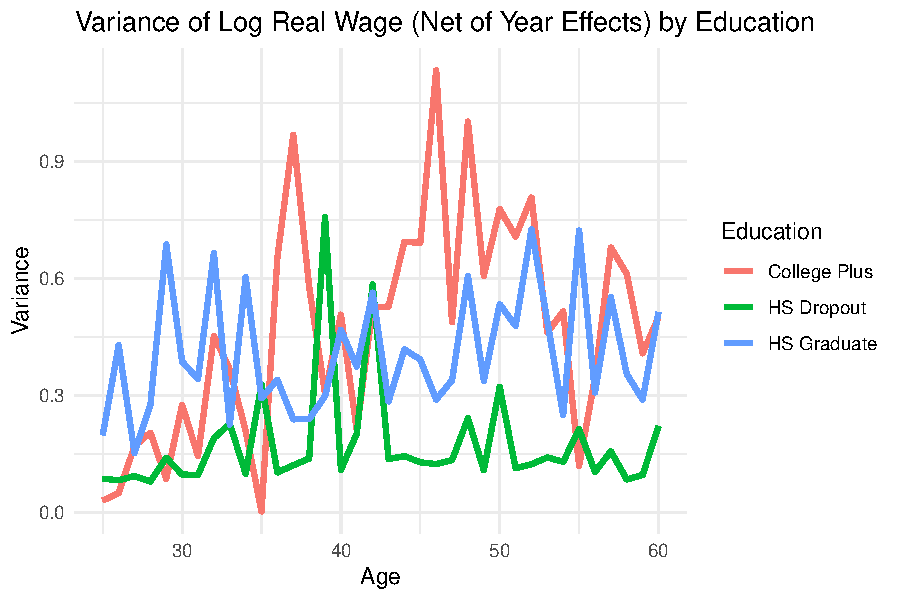
\includegraphics[width=0.8\textwidth]{~/SchoolWork/Y2S1/Macro/PSets/ps1/output/var_wage_age_educ.pdf}
    \caption{Variance of Wages by Age (Stratified by Education)}
\end{figure}

Variance of wages is highest for college graduates, perhaps becuase there is a very wide range of wages for college graduates, as well as the fact that post-grad degree
holders are included in this group, and thus have a much higher variance in wages.

\subsection*{Table of Data Facts}

\begin{tabular}{||l|c|c|c|c|c|c||}
  Year & Group & Category & Sample Size & Observations & College (\%) & White Collar (\%) \\
  \hline\hline \\
  1999 & All & All & 1847 & 3795 & 22.6 & 57 \\
  & Education & HS Dropout & 807 & 1288 & & \\
  & Education & HS Grad & 873 & 1288 & & \\
  & Education & College + & 873 & 1288 & & \\
  & Industry & Blue Collar & 507 & 629 & & \\
  & Industry & White Collar & 507 & 629 & & \\
  & Wealth & Bottom 25\% & 1847 & 3795 & & \\
  & Wealth & Middle 50\% & 1847 & 3795 & & \\
  & Wealth & Top 25\% & 1847 & 3795 & & \\
  2001 & All & All & 1855 & 4078 & 24.1 & 55.7 \\
  & Education & HS Dropout & 883 & 1358 & & \\
  & Education & HS Grad & 883 & 1358 & & \\
  & Education & College + & 883 & 1358 & & \\
  & Industry & Blue Collar & 541 & 646 & & \\
  & Industry & White Collar & 541 & 646 & & \\
  & Wealth & Bottom 25\% & 1855 & 4078 & & \\
  & Wealth & Middle 50\% & 1855 & 4078 & &
  & Wealth & Top 25\% & 1855 & 4078 & & \\
  2003 & All & All & 1844 & 4209 & 24.1 & 28.2 \\
  & Education & HS Dropout & 892 & 1384 & & \\
  & Education & HS Grad & 892 & 1384 & & \\
  & Education & College + & 892 & 1384 & & \\
  & Industry & Blue Collar & 597 & 773 & & \\
  & Industry & White Collar & 597 & 773 & & \\
  & Wealth & Bottom 25\% & 1844 & 4209 & & \\
  & Wealth & Middle 50\% & 1844 & 4209 & & \\
  & Wealth & Top 25\% & 1844 & 4209 & & \\
  2005 & All & All & 1814 & 4231 & 22.1 & 26.4 \\
  & Education & HS Dropout & 872 & 1380 & & \\
  & Education & HS Grad & 872 & 1380 & & \\
  & Education & College + & 872 & 1380 & & \\
  & Industry & Blue Collar & 607 & 793 & & \\
  & Industry & White Collar & 607 & 793 & & \\
  & Wealth & Bottom 25\% & 1814 & 4231 & & \\
  & Wealth & Middle 50\% & 1814 & 4231 & & \\
  & Wealth & Top 25\% & 1814 & 4231 & & \\
  2007 & All & All & 1799 & 4349 & 21.2 & 25.0 \\
  & Education & HS Dropout & 866 & 1387 & & \\
  & Education & HS Grad & 866 & 1387 & & \\
  & Education & College + & 866 & 1387 & & \\
  & Industry & Blue Collar & 642 & 839 & & \\
  & Industry & White Collar & 642 & 839 & & \\
  & Wealth & Bottom 25\% & 1799 & 4349 & & \\
  & Wealth & Middle 50\% & 1799 & 4349 & & \\
  & Wealth & Top 25\% & 1799 & 4349 & & \\
\end{tabular}
\begin{tabular}{||l|c|c|c|c|c|c||}
  Year & Group & Category & Sample Size & Observations & College (\%) & White Collar (\%) \\
  \hline\hline \\
  2009 & All & All & 1767 & 4421 & 29.3 & 26.2 \\
  & Education & HS Dropout & 929 & 1522 & & \\
  & Education & HS Grad & 929 & 1522 & & \\
  & Education & College + & 929 & 1522 & & \\
  & Industry & Blue Collar & 627 & 856 & & \\
  & Industry & White Collar & 627 & 856 & & \\
  & Wealth & Bottom 25\% & 1767 & 4421 & & \\
  & Wealth & Middle 50\% & 1767 & 4421 & & \\
  & Wealth & Top 25\% & 1767 & 4421 & & \\
  2011 & All & All & 1713 & 4441 & 28.0 & 27.5 \\
  & Education & HS Dropout & 921 & 1536 & & \\
  & Education & HS Grad & 921 & 1536 & & \\
  & Education & College + & 921 & 1536 & & \\
  & Industry & Blue Collar & 557 & 777 & & \\
  & Industry & White Collar & 557 & 777 & & \\
  & Wealth & Bottom 25\% & 1713 & 4441 & & \\
  & Wealth & Middle 50\% & 1713 & 4441 & & \\
  & Wealth & Top 25\% & 1713 & 4441 & & \\
  2013 & All & All & 1701 & 4475 & 27.8 & 27.6 \\
  & Education & HS Dropout & 928 & 1555 & & \\
  & Education & HS Grad & 928 & 1555 & & \\
  & Education & College + & 928 & 1555 & & \\
  & Industry & Blue Collar & 566 & 782 & & \\
  & Industry & White Collar & 566 & 782 & & \\
  & Wealth & Bottom 25\% & 1701 & 4475 & & \\
  & Wealth & Middle 50\% & 1701 & 4475 & & \\
  & Wealth & Top 25\% & 1701 & 4475 & & \\
  2015 & All & All & 1650 & 4365 & 27.3 & 28.1 \\
  & Education & HS Dropout & 921 & 1512 & & \\
  & Education & HS Grad & 921 & 1512 & & \\
  & Education & College + & 921 & 1512 & & \\
  & Industry & Blue Collar & 566 & 782 & & \\
  & Industry & White Collar & 566 & 782 & & \\
  & Wealth & Bottom 25\% & 1650 & 4365 & & \\
  & Wealth & Middle 50\% & 1650 & 4365 & & \\
  & Wealth & Top 25\% & 1650 & 4365 & & \\
  2017 & All & All & 1908 & 4684 & 49.3 & NA \\
  & Education & HS Dropout & 880 & 1399 & & \\
  & Education & HS Grad & 880 & 1399 & & \\
  & Education & College + & 880 & 1399 & & \\
  & Industry & Blue Collar & 551 & 764 & & \\
  & Industry & White Collar & 551 & 764 & & \\
  & Wealth & Bottom 25\% & 1908 & 4684 & & \\
  & Wealth & Middle 50\% & 1908 & 4684 & & \\
  & Wealth & Top 25\% & 1908 & 4684 & & \\
\end{tabular}

\end{document}
